% !TeX spellcheck = en_B
% !TeX encoding = UTF-8 %%%These comments just make you look like you know what you're doing
\documentclass[8pt]{beamer}  %%% Specifies the class, with 8pt font size

\usepackage[utf8]{inputenc}
\usetheme[block=fill,progressbar=foot,background=light]{metropolis}     
\usepackage[english]{babel}
\usepackage{csquotes}       
\usepackage[T1]{fontenc}        
\usepackage{booktabs}
\usepackage{pgfgantt}
\usepackage{pifont}
\usepackage{adfbullets}
\usepackage{enumitem}
\usepackage{amsmath}   
\usepackage{tikz}
\usepackage{lipsum}
\usepackage{amssymb}
\usepackage{amsfonts}
\usepackage{mathrsfs}   
\usepackage{graphicx}
\usepackage{adjustbox}
\usepackage{varioref}
\usepackage{probsoln}
\usepackage{attachfile2}
\usepackage{pgfplots}
\pgfplotsset{compat=newest}
\usepackage[]{hyperref} 
\graphicspath{{Graphics/}}
\usepackage{multirow,array}
\usepackage{colortbl}
\definecolor{aa}{RGB}{255, 124, 0}
\definecolor{cc}{RGB}{230, 230, 230}    
\usebackgroundtemplate{%
\tikz[overlay,remember picture]{\node[scale=80,opacity=0.03, at=(current page.south east)] {\adfbullet{9}};}}
  
\date[\today]{\today}

\usepackage{comment}
\usepackage{varwidth}

\newcommand{\mat}[4]{\left(\begin{array}{cc} #1 & #2 \\ #3 & #4 \\ \end{array}\right)}
\newcommand{\Q}{\mathbb{Q}}
\newcommand{\R}{\mathbb{R}}
\newcommand{\Z}{\mathbb{Z}}
\newcommand{\sol}[2][+]{
	\tikz[baseline]{\node[color=aa,fill=cc,rectangle,draw,anchor=base] {  {\onslide<#1->{#2}}  };}
}

\usetikzlibrary{positioning}
\usetikzlibrary{tikzmark}
\usetikzlibrary{shadings}
\usetikzlibrary{through}

\def\height{0.8cm}
\def\width{1.2cm}
\newcommand{\keynode}[6]{\node[minimum height=\height,minimum width=\width,draw,rectangle,color=aa,fill=cc] (#3) at (#1,#2) {};
	\node[rectangle,minimum height=\height/2,minimum width=\width,above,color=aa] at (#3) {#3};
	\node[draw,rectangle,minimum height=\height/2,minimum width=\width/3,below,color=aa,fill=cc,inner sep =0cm] at (#3) {\footnotesize#4};
	\node[draw,rectangle,minimum height=\height/2,minimum width=\width/3,below,xshift=\height/2,color=aa,fill=cc,inner sep=0cm] at (#3) {\footnotesize#5};
	\node[draw,rectangle,minimum height=\height/2,minimum width=\width/3,below,xshift=-\height/2,color=aa,fill=cc,inner sep=0cm] at (#3) {\footnotesize#6}; }

\newenvironment{gantt}[3]{\begin{ganttchart}[#1,bar height=.6,bar top shift=.2,title/.style=  {draw=none},y unit chart=0.6cm,y unit title = 0.6cm,include title in canvas=false,group/.append style={draw=black,dashed},bar/.append style={fill=aa},inline,hgrid=true,Float1/.style={bar/.append style={fill=none,dashed},bar height=.8,bar top shift=0.1}]{#2}{#3}}{\end{ganttchart}}

\newenvironment{nicetable}[1]{\setlength\arrayrulewidth{0.5mm}
			\arrayrulecolor{white}
			\begin{tabular}{#1}}{\end{tabular}}
		
\setlist[itemize,1]{label={\color{aa}\huge\adfbullet{9}}}
\setlist[itemize, 2]{label={\color{aa}\large\adfbullet{9}}}

\newcommand\reshist{}
\def\reshist(#1)#2(#3)#4(#5)%
{\draw (axis cs:#1) rectangle (axis cs:#3) node [midway] {#5};} %%%adds the general preamble

\title{{\color{aa}\Huge\adfbullet{9}} Redes Neuronales} %%%Title and subtitle
\subtitle{Introducción \textattachfile{Template.tex}{(TeX)}} %%%This embeds the tikz source code into the resulting pdf...
\date{Enero-Julio 2021}
\begin{document}

\frame{\titlepage} %%%Makes titlepage

\setlength{\abovedisplayskip}{0pt}
\setlength{\belowdisplayskip}{0pt}
\setlength{\abovedisplayshortskip}{0pt}
\setlength{\belowdisplayshortskip}{0pt}  %%%Compresses math
%%%%%%%%%%%%%%%%%%%%%%%%%%%%%%%%%%%%%%%%%%%%%%%%%%%%%%%%%%%%%%%%%%%%%%%%%

\begin{frame}{Contenido} 
   \tableofcontents
\end{frame}
%%%%%%%%%%%%%%%%%%%%%%%%%%%%%%%%%%%%%%%%%%%%%%%%%%%%%%%%%%%%%%%%%%%%%%
\section{Introducción}
\subsection{Contextualización}
\begin{frame}{Regresión lógistica}
	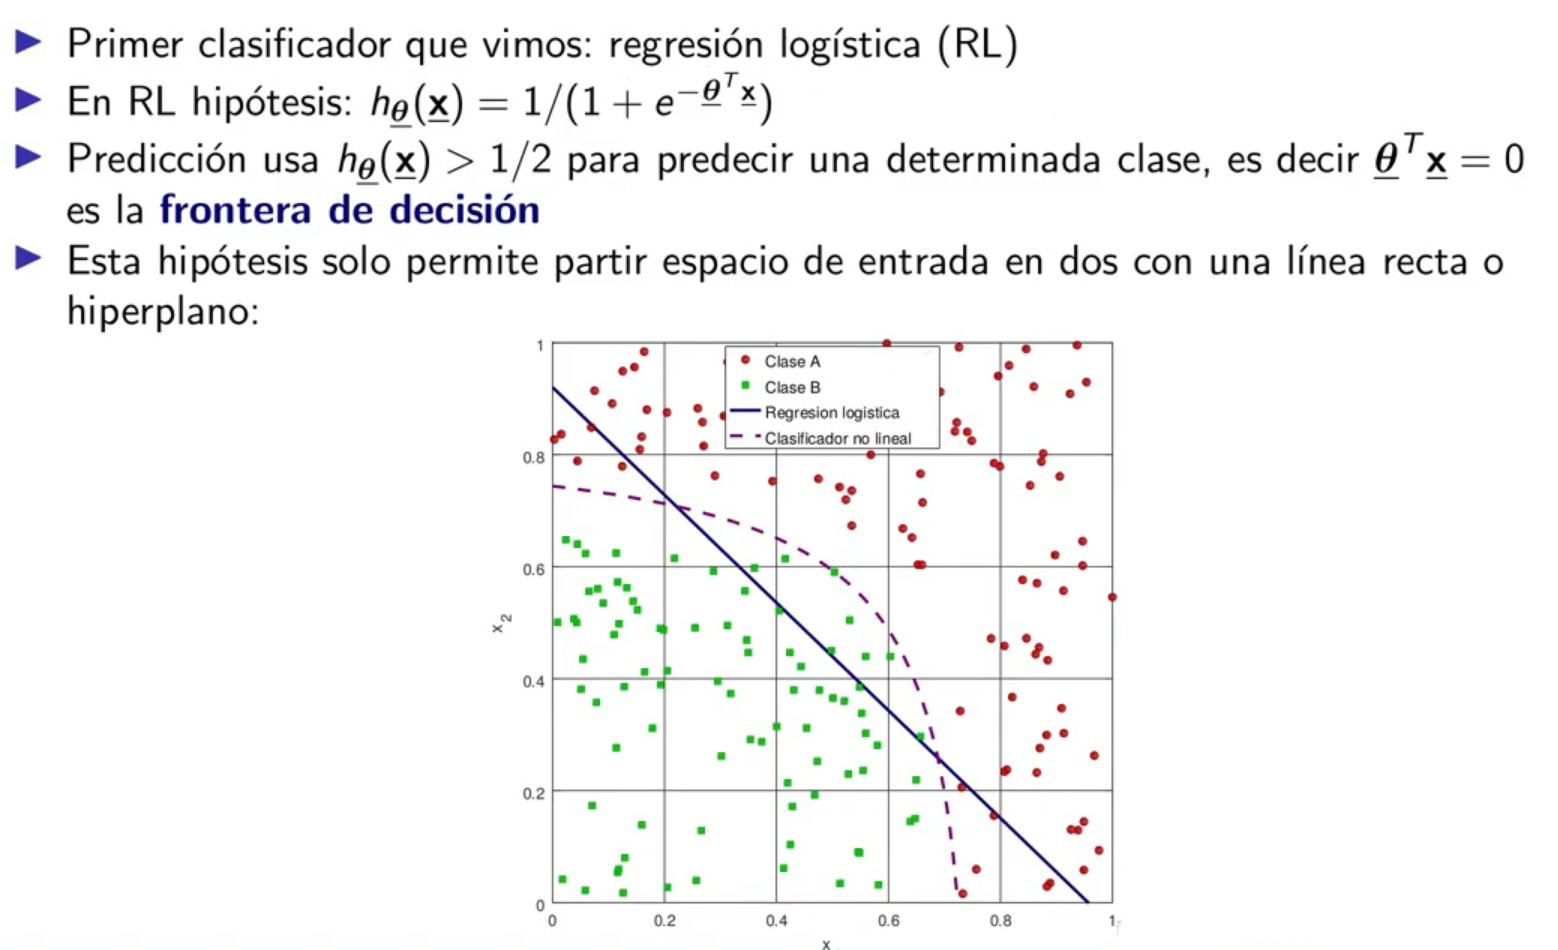
\includegraphics[width=\textwidth]{im1}
\end{frame}
%%%%%%%%%%%%%%%%%%%%%%%%%%%%%%%%%%%%%%%%%%%%%%%%%%%%%%%%%%%%%%%%%%%%%%%%%
\begin{frame}{Regresión lógistica}
	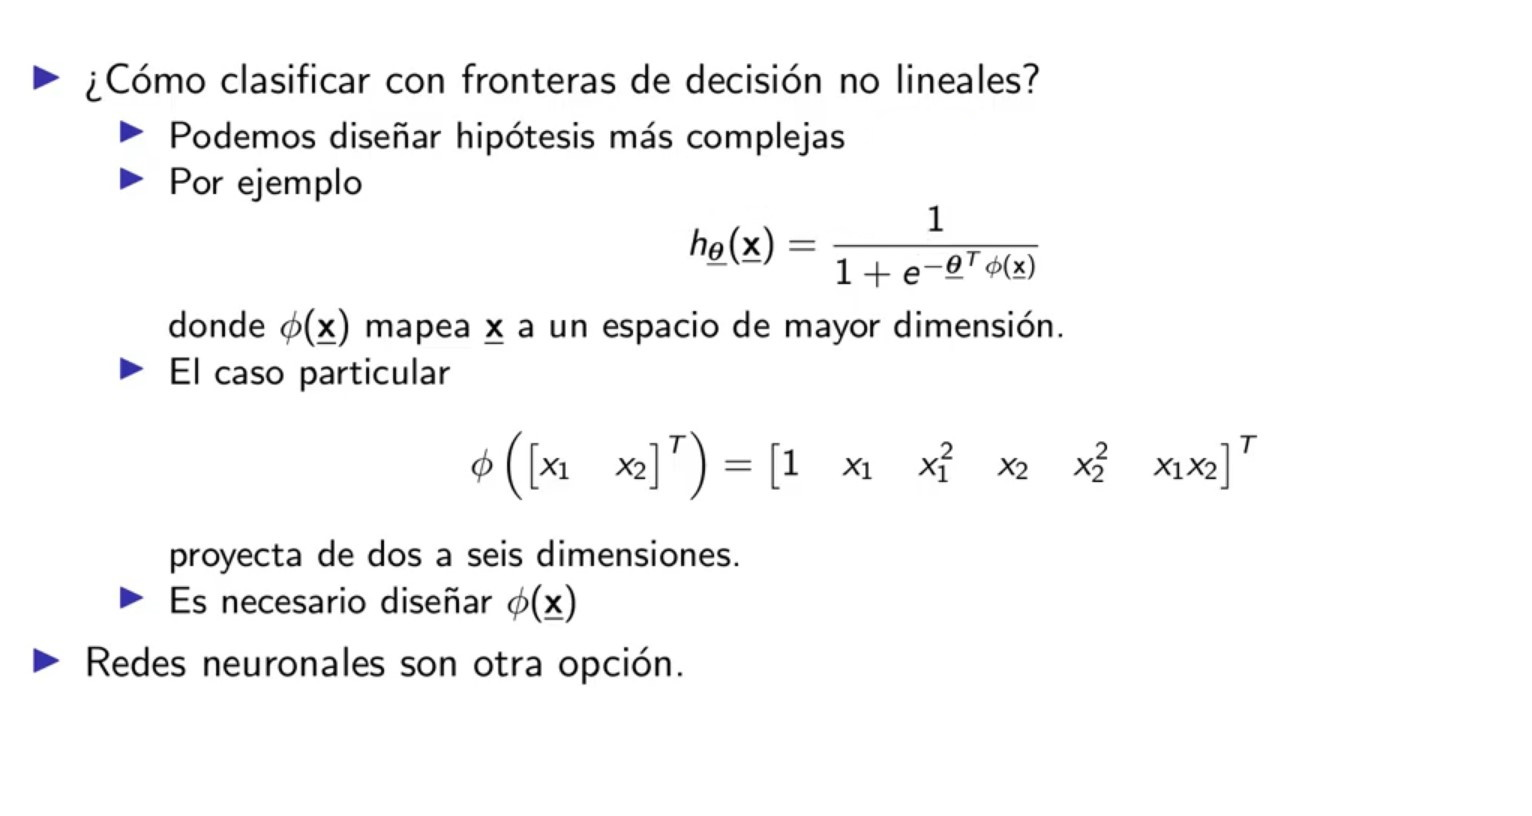
\includegraphics[width=\textwidth]{im2}
\end{frame}
%%%%%%%%%%%%%%%%%%%%%%%%%%%%%%%%%%%%%%%%%%%%%%%%%%%%%%%%%%%%%%%%%%%%%%%%%
\subsection{Inspiración biológica}
\begin{frame}{Redes neuronales biológicas}
	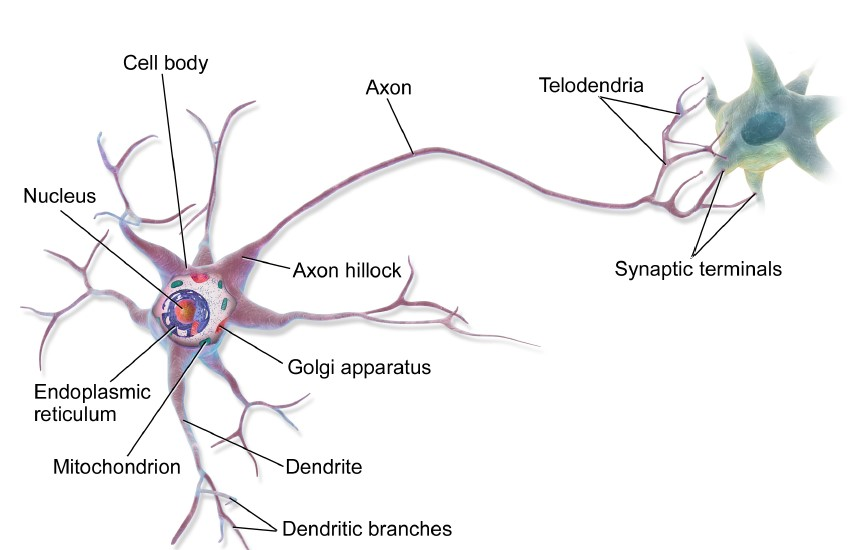
\includegraphics[width=\textwidth]{neurona}
\end{frame}
%%%%%%%%%%%%%%%%%%%%%%%%%%%%%%%%%%%%%%%%%%%%%%%%%%%%%%%%%%%%%%%%%%%%%%%%%
\begin{frame}{Redes neuronales biológicas}
	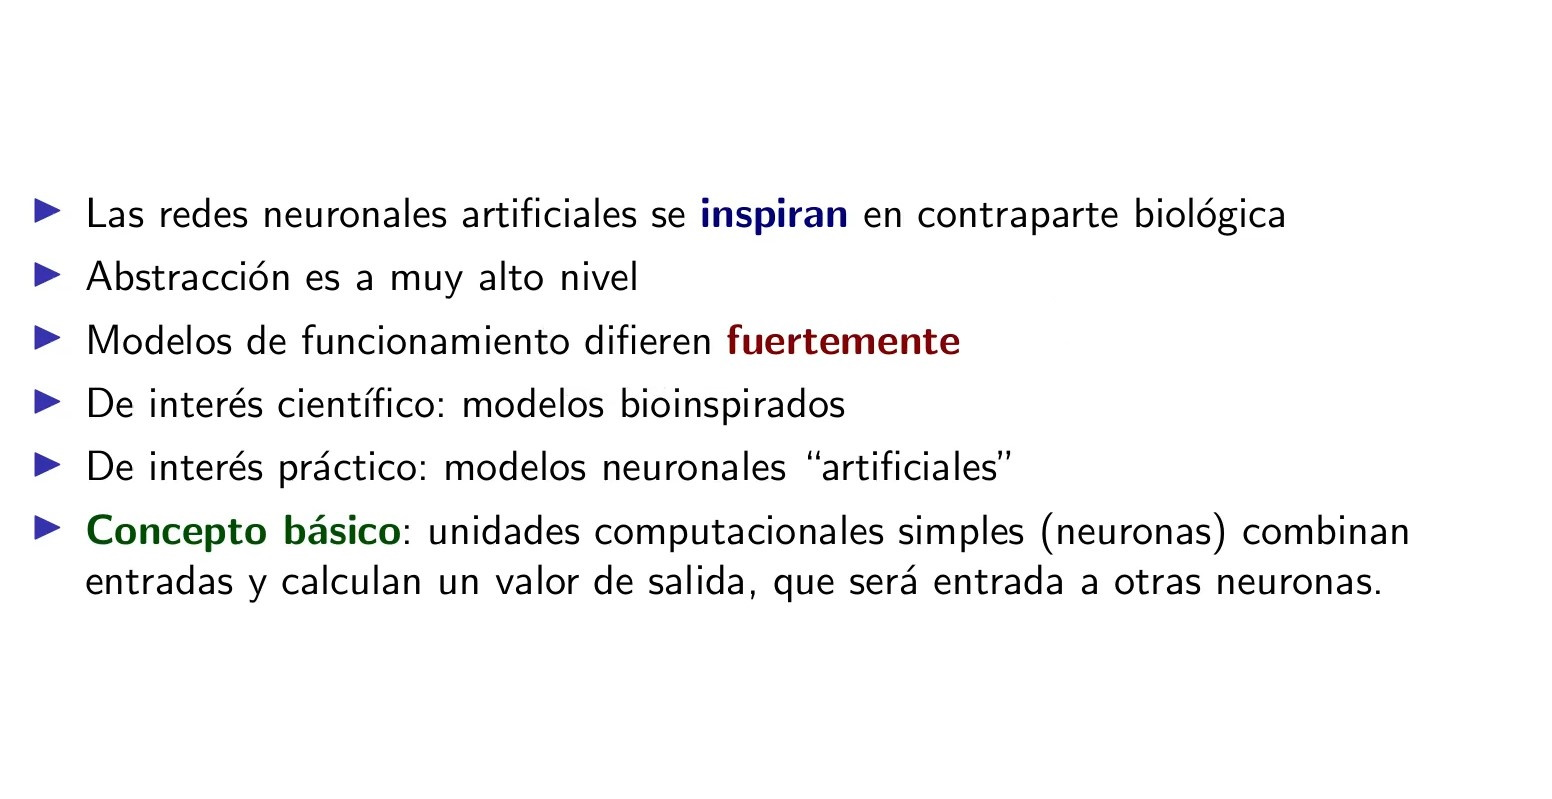
\includegraphics[width=\textwidth]{im3}
\end{frame}
%%%%%%%%%%%%%%%%%%%%%%%%%%%%%%%%%%%%%%%%%%%%%%%%%%%%%%%%%%%%%%%%%%%%%%%%%
\subsection{Nuerona Artificial}
\begin{frame}{Perceptron }
	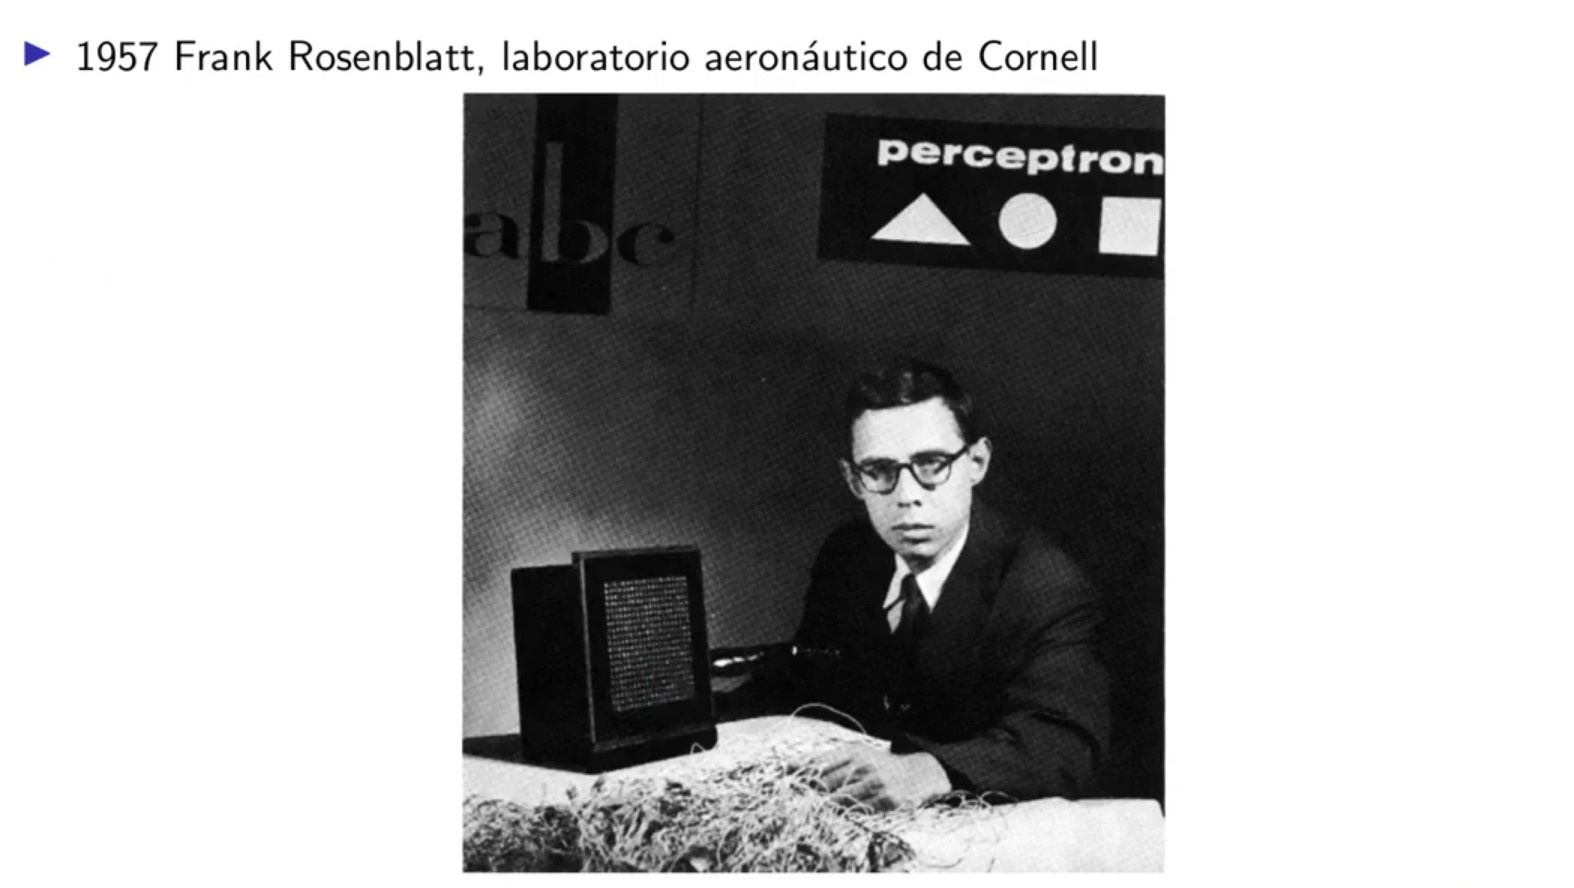
\includegraphics[width=\textwidth]{im4}
\end{frame}
%%%%%%%%%%%%%%%%%%%%%%%%%%%%%%%%%%%%%%%%%%%%%%%%%%%%%%%%%%%%%%%%%%%%%%%%%
\begin{frame}{Perceptron }
	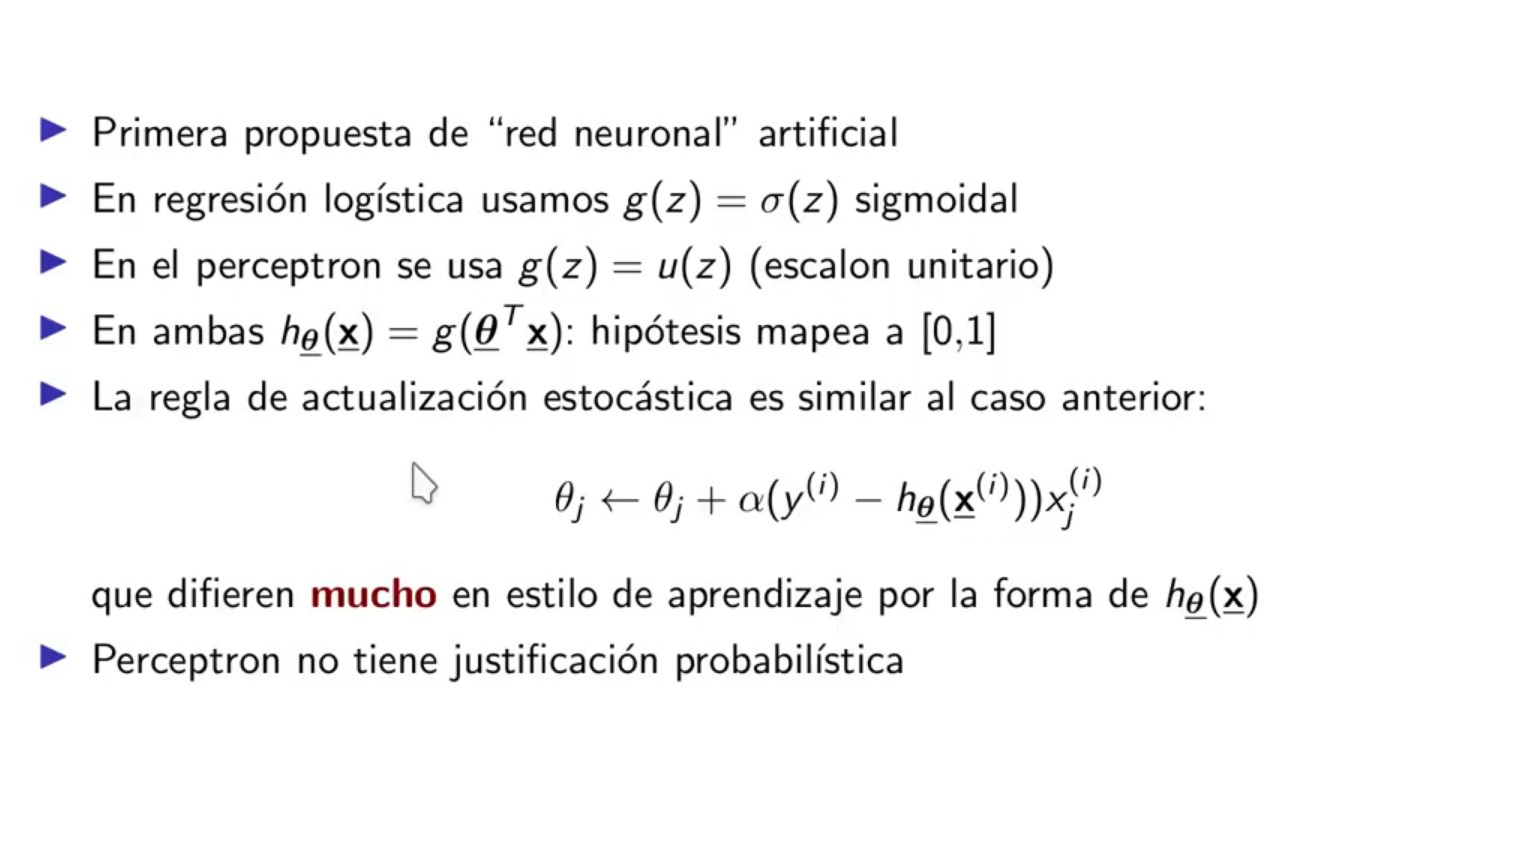
\includegraphics[width=\textwidth]{im5}
\end{frame}
%%%%%%%%%%%%%%%%%%%%%%%%%%%%%%%%%%%%%%%%%%%%%%%%%%%%%%%%%%%%%%%%%%%%%%%%%
\begin{frame}{Nuerona arificial}
	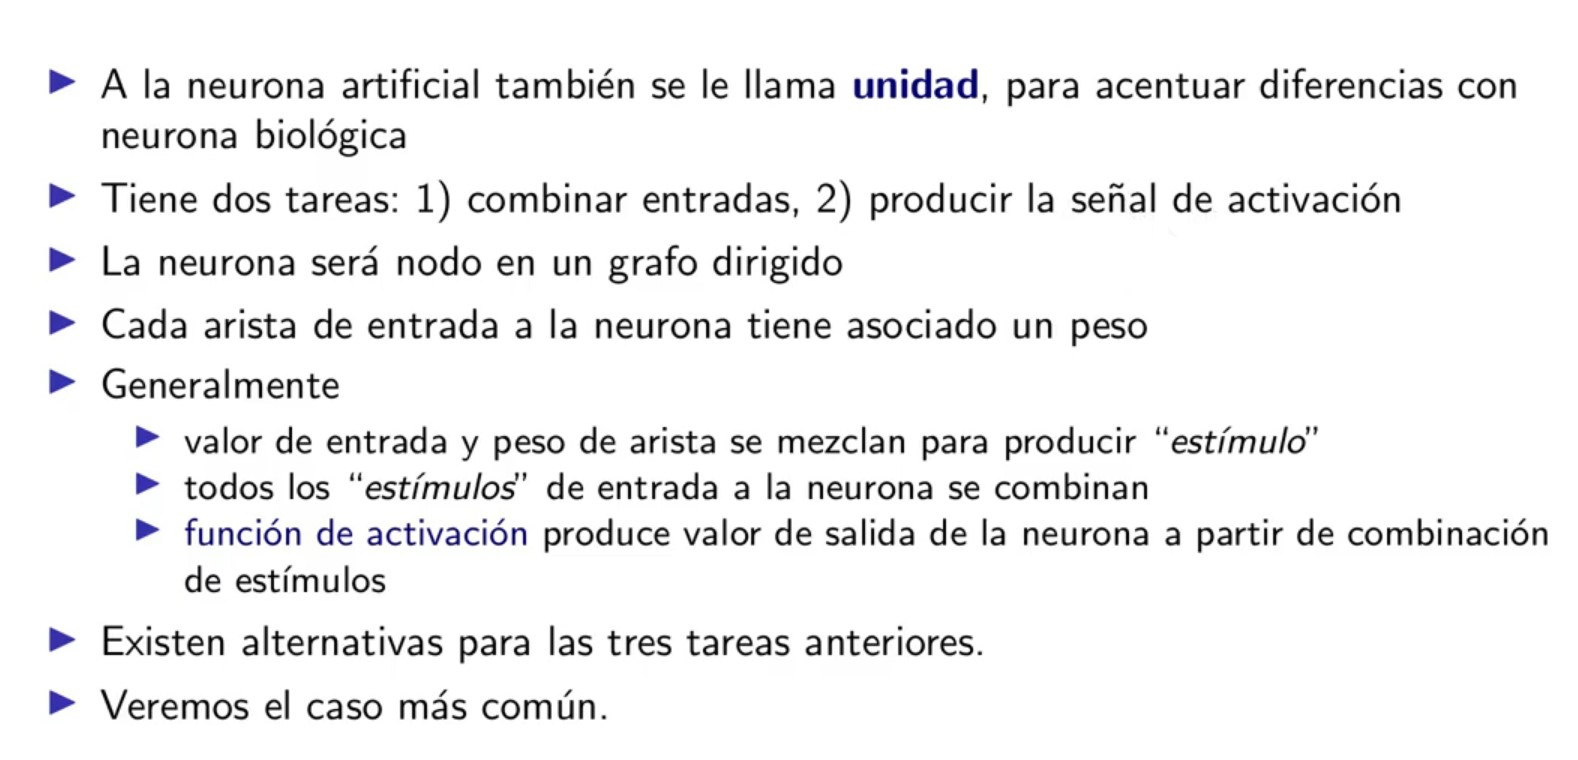
\includegraphics[width=\textwidth]{im6}
\end{frame}

%%%%%%%%%%%%%%%%%%%%%%%%%%%%%%%%%%%%%%%%%%%%%%%%%%%%%%%%%%%%%%%%%%%%%%%%%
\begin{frame}{Modelo nuerona artificial}
	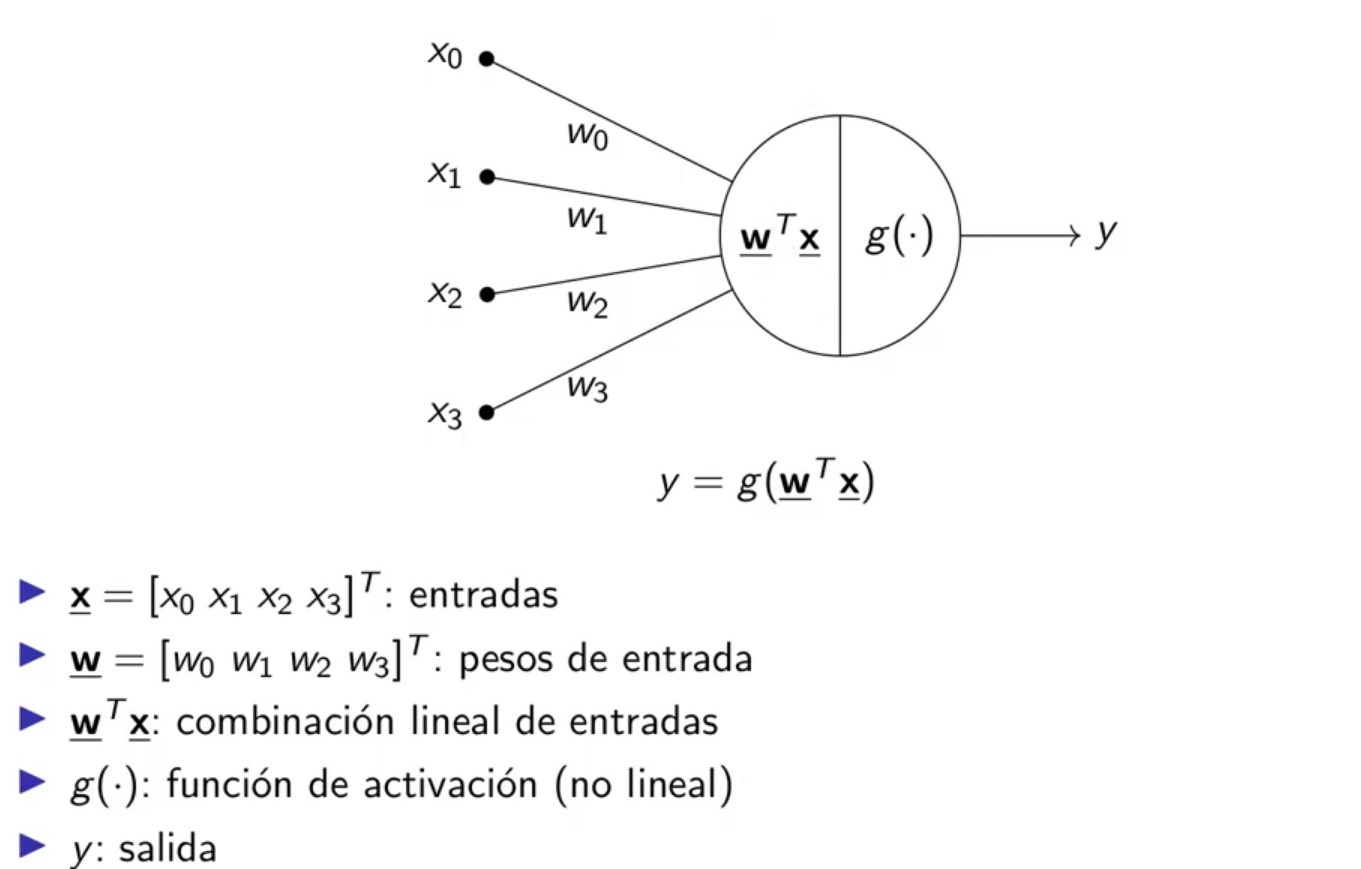
\includegraphics[width=\textwidth]{im7}
\end{frame}
%%%%%%%%%%%%%%%%%%%%%%%%%%%%%%%%%%%%%%%%%%%%%%%%%%%%%%%%%%%%%%%%%%%%%%%%%
\begin{frame}{Modelo nuerona artificial}
	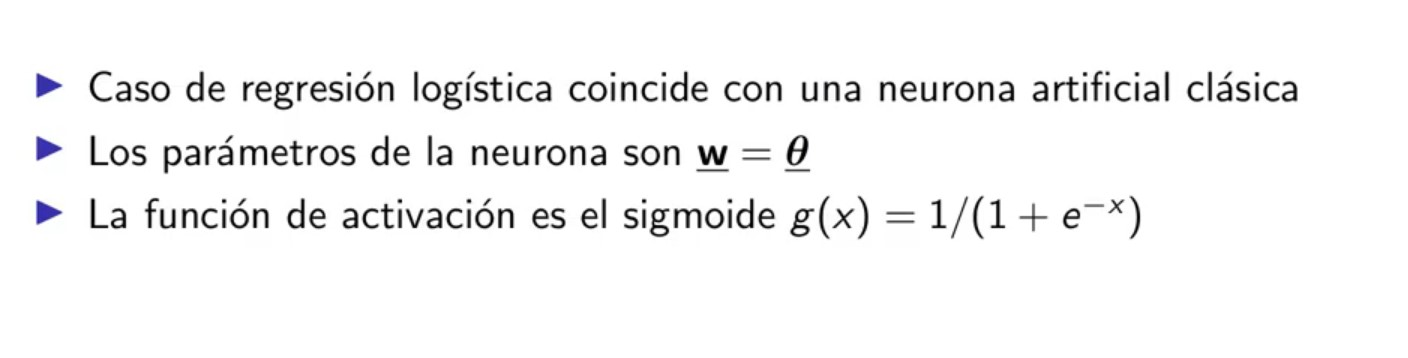
\includegraphics[width=\textwidth]{im8}
\end{frame}
%%%%%%%%%%%%%%%%%%%%%%%%%%%%%%%%%%%%%%%%%%%%%%%%%%%%%%%%%%%%%%%%%%%%%%%%%
\section{Red Neuronal Artificial}
\subsection{Hipótesis}
\begin{frame}{Red Neuronal Artificial}
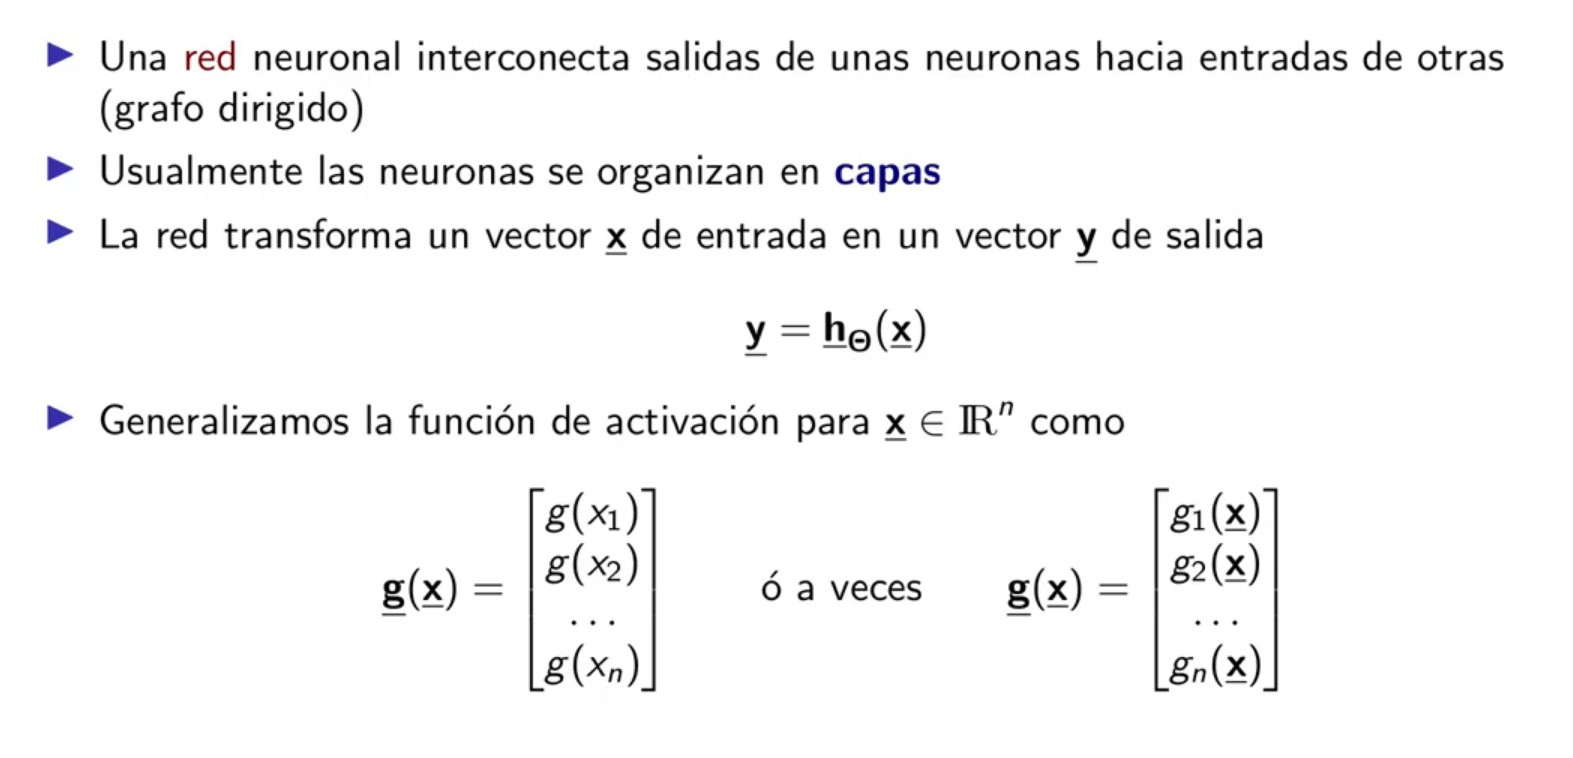
\includegraphics[width=\textwidth]{im9}
\end{frame}

%%%%%%%%%%%%%%%%%%%%%%%%%%%%%%%%%%%%%%%%%%%%%%%%%%%%%%%%%%%%%%%%%%%%%%%%%
\subsection{Capas}
\begin{frame}{Red Neuronal Artificial}
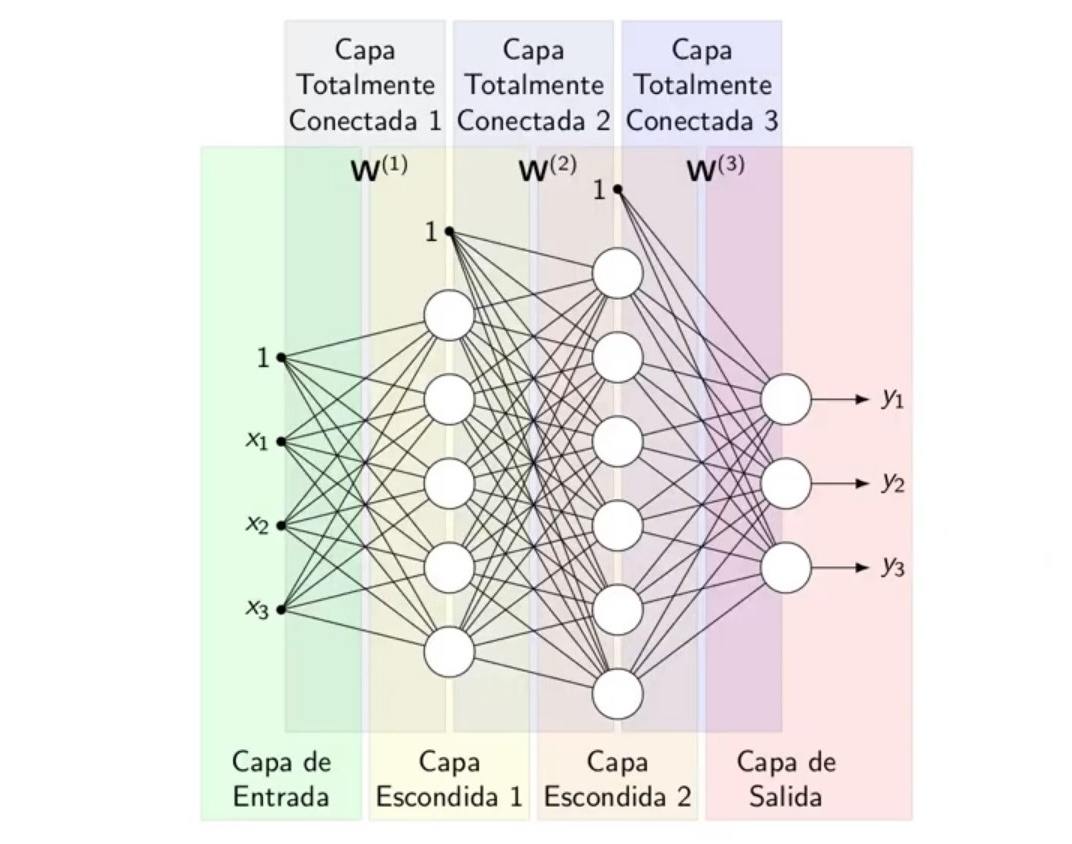
\includegraphics[width=\textwidth]{im10}
\end{frame}
%%%%%%%%%%%%%%%%%%%%%%%%%%%%%%%%%%%%%%%%%%%%%%%%%%%%%%%%%%%%%%%%%%%%%%%%%
\begin{frame}{Red Neuronal Artificial}
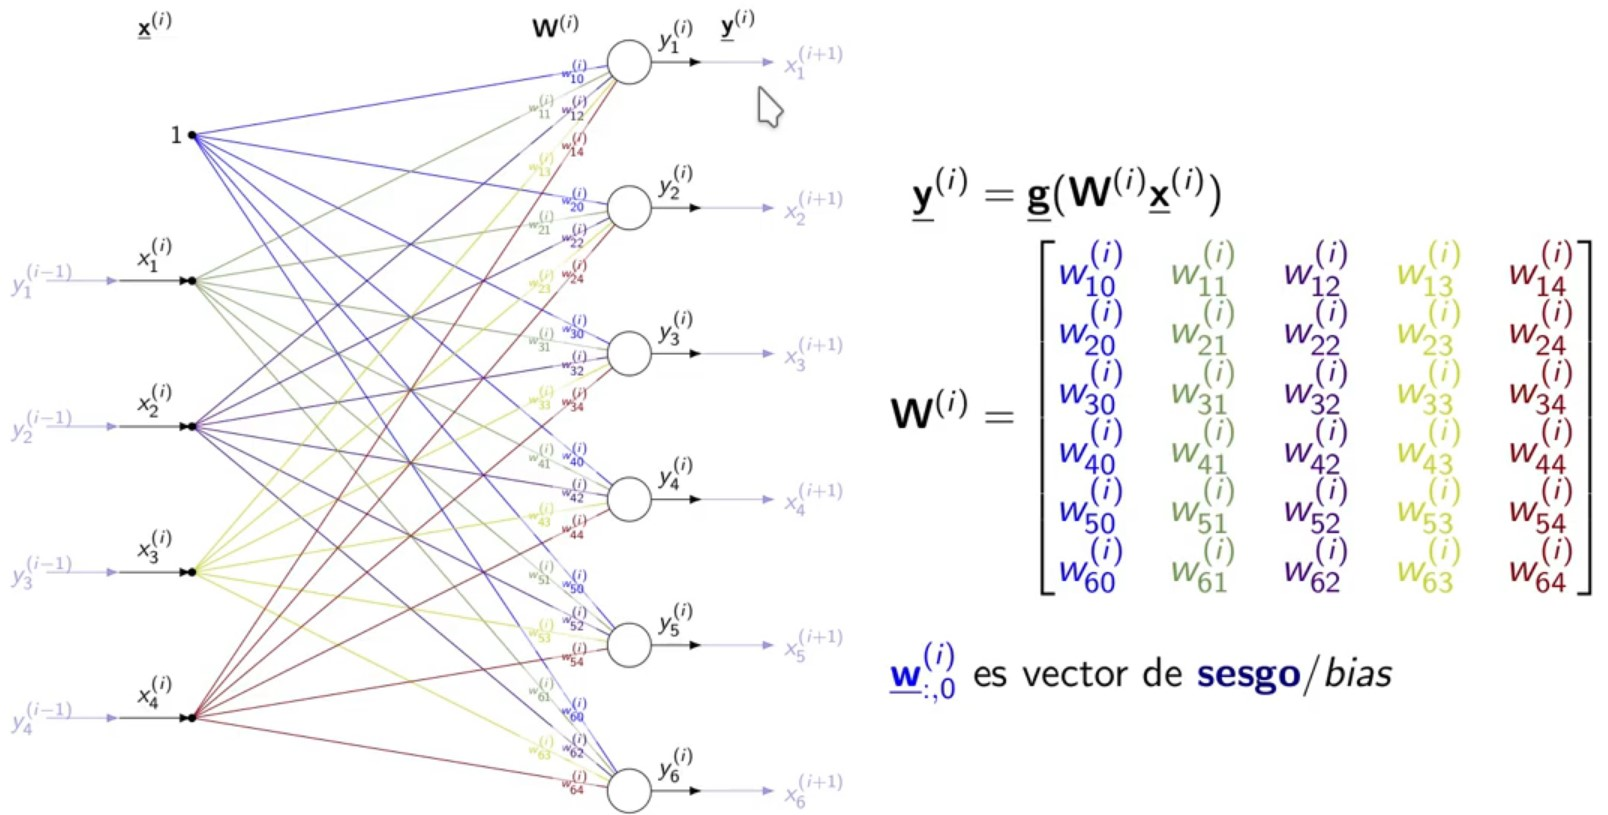
\includegraphics[width=\textwidth]{im11}
\end{frame}
%%%%%%%%%%%%%%%%%%%%%%%%%%%%%%%%%%%%%%%%%%%%%%%%%%%%%%%%%%%%%%%%%%%%%%%%%
\begin{frame}{Red Neuronal Artificial}
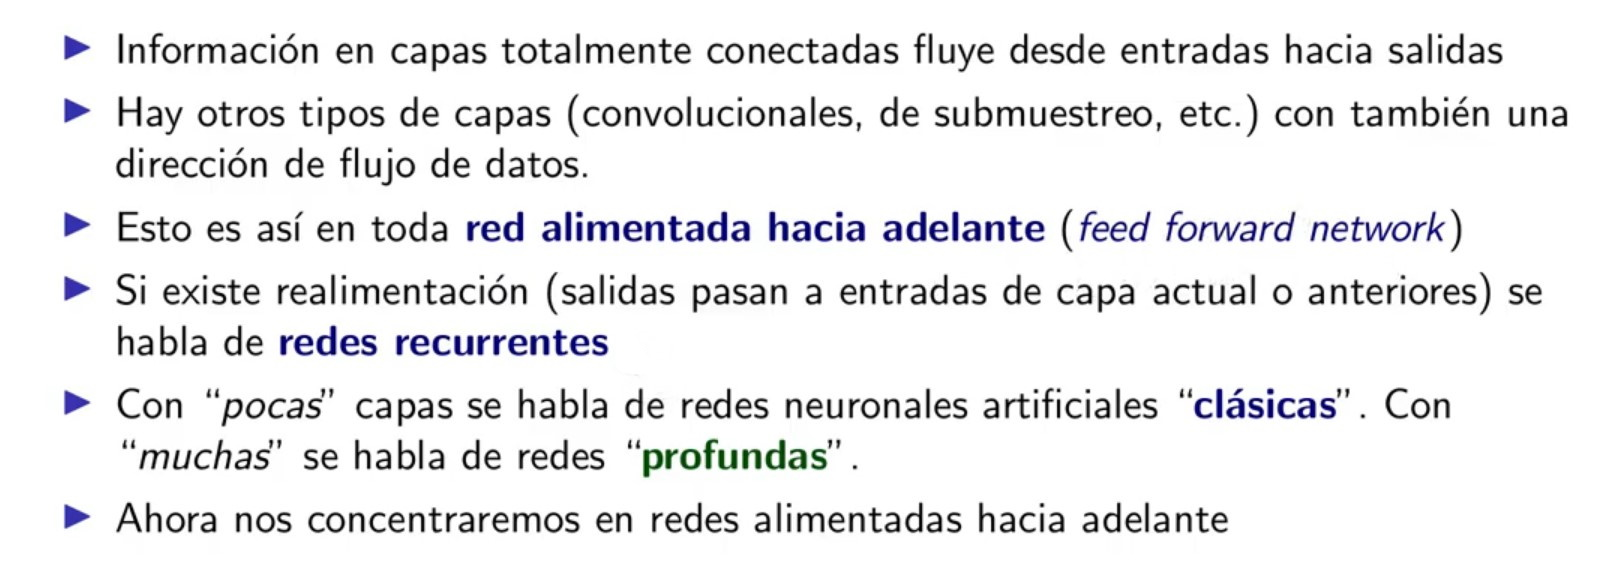
\includegraphics[width=\textwidth]{im12}
\end{frame}
%%%%%%%%%%%%%%%%%%%%%%%%%%%%%%%%%%%%%%%%%%%%%%%%%%%%%%%%%%%%%%%%%%%%%%%%%
\begin{frame}{Red Neuronal Artificial}
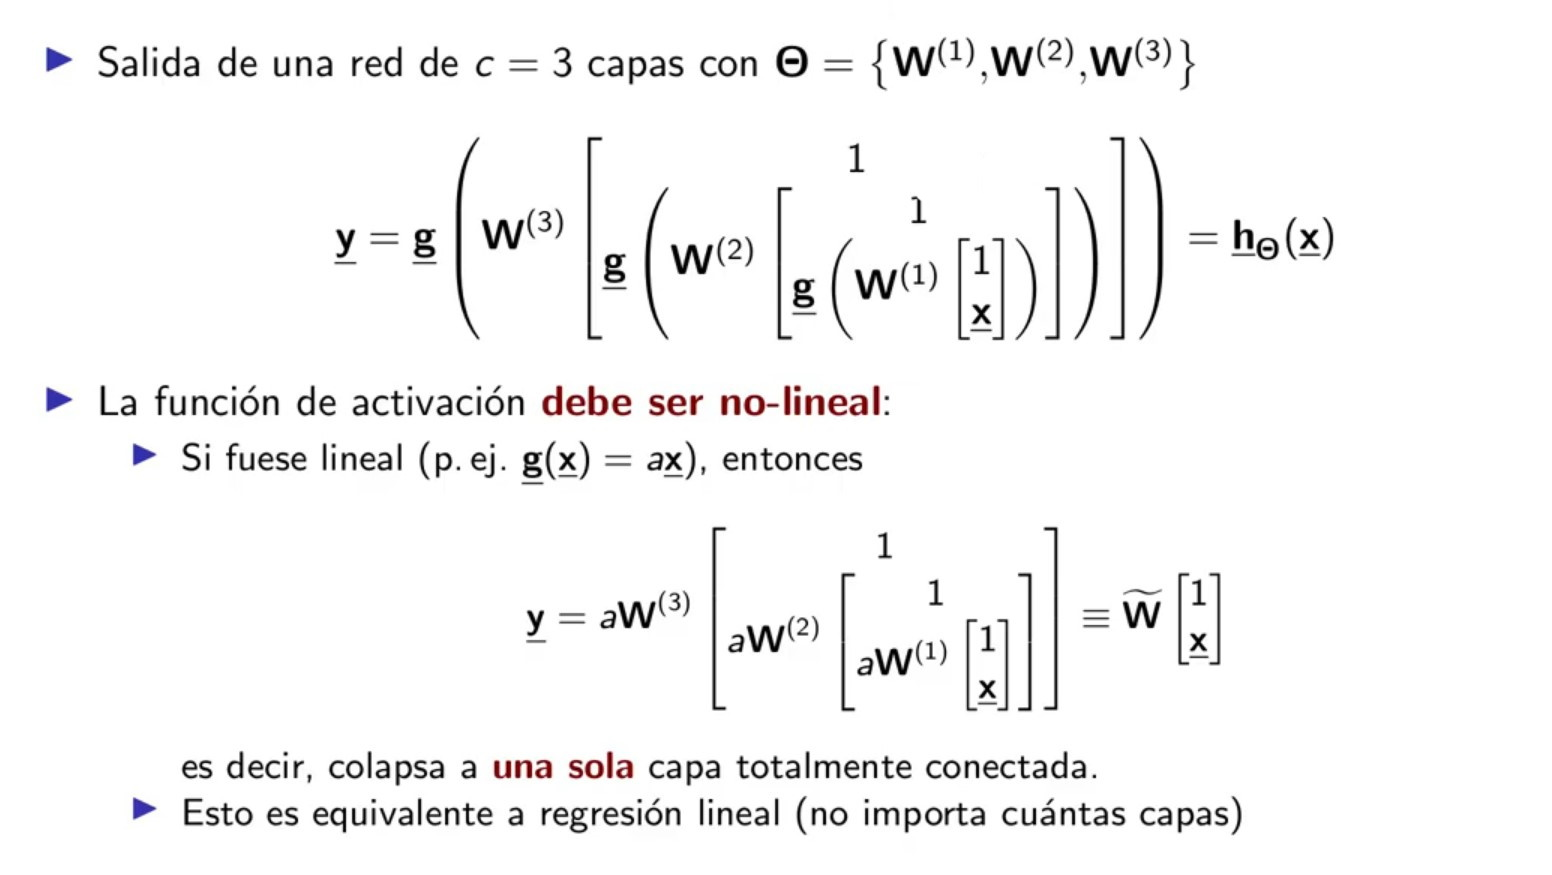
\includegraphics[width=\textwidth]{im13}
\end{frame}
%%%%%%%%%%%%%%%%%%%%%%%%%%%%%%%%%%%%%%%%%%%%%%%%%%%%%%%%%%%%%%%%%%%%%%%%%
\begin{frame}{Red Neuronal Artificial}
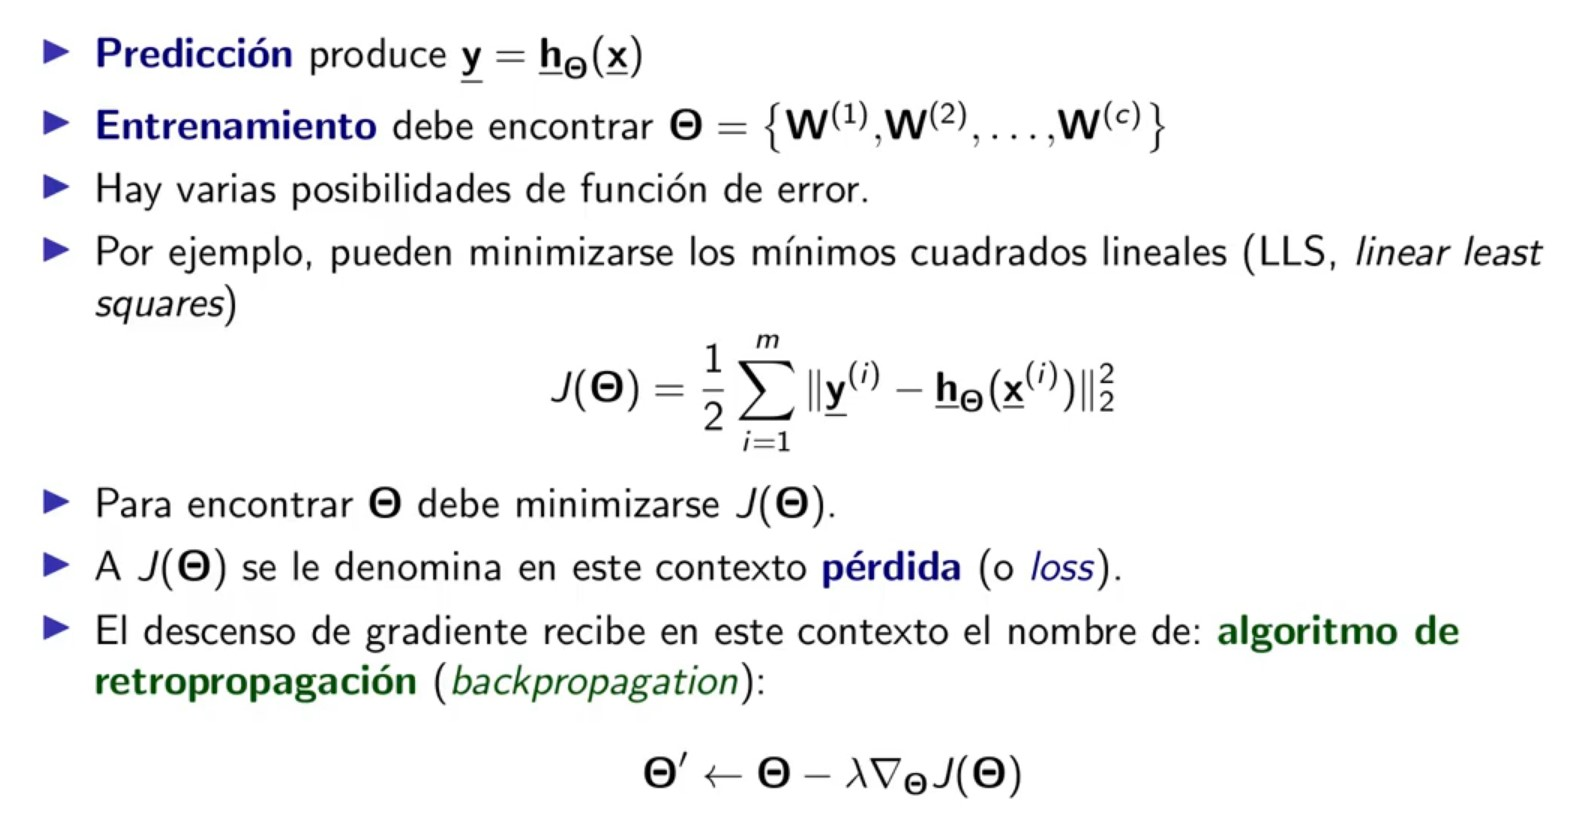
\includegraphics[width=\textwidth]{im14}
\end{frame}
%%%%%%%%%%%%%%%%%%%%%%%%%%%%%%%%%%%%%%%%%%%%%%%%%%%%%%%%%%%%%%%%%%%%%%%%%
\begin{frame}{Red Neuronal Artificial}
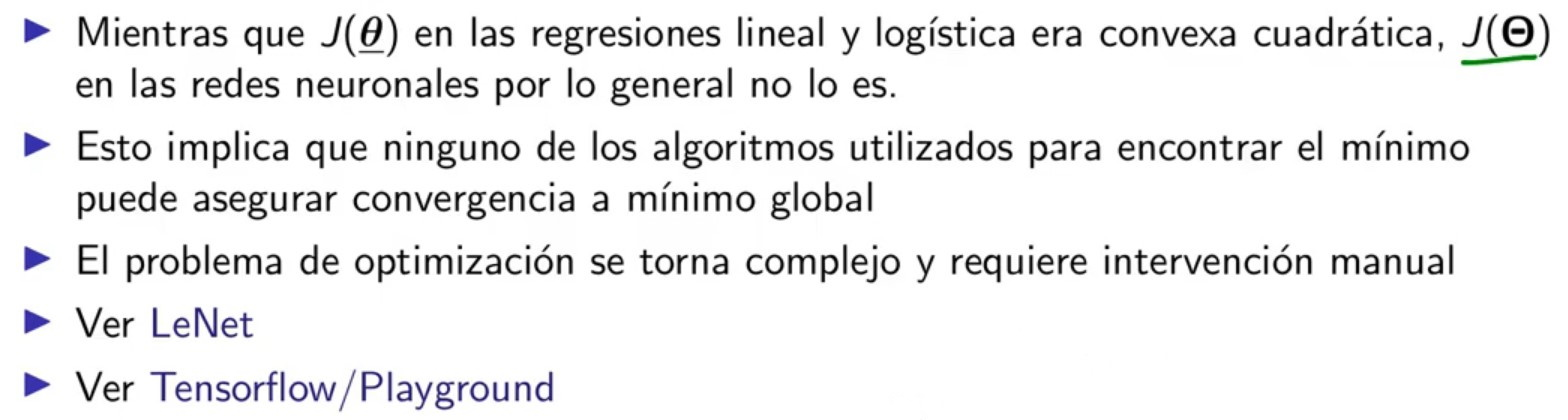
\includegraphics[width=\textwidth]{im15}
\end{frame}
%%%%%%%%%%%%%%%%%%%%%%%%%%%%%%%%%%%%%%%%%%%%%%%%%%%%%%%%%%%%%%%%%%%%%%%%%


\end{document}
